\subsection{Esquema de caja negra}

\begin{figure}[H]
  \centering
  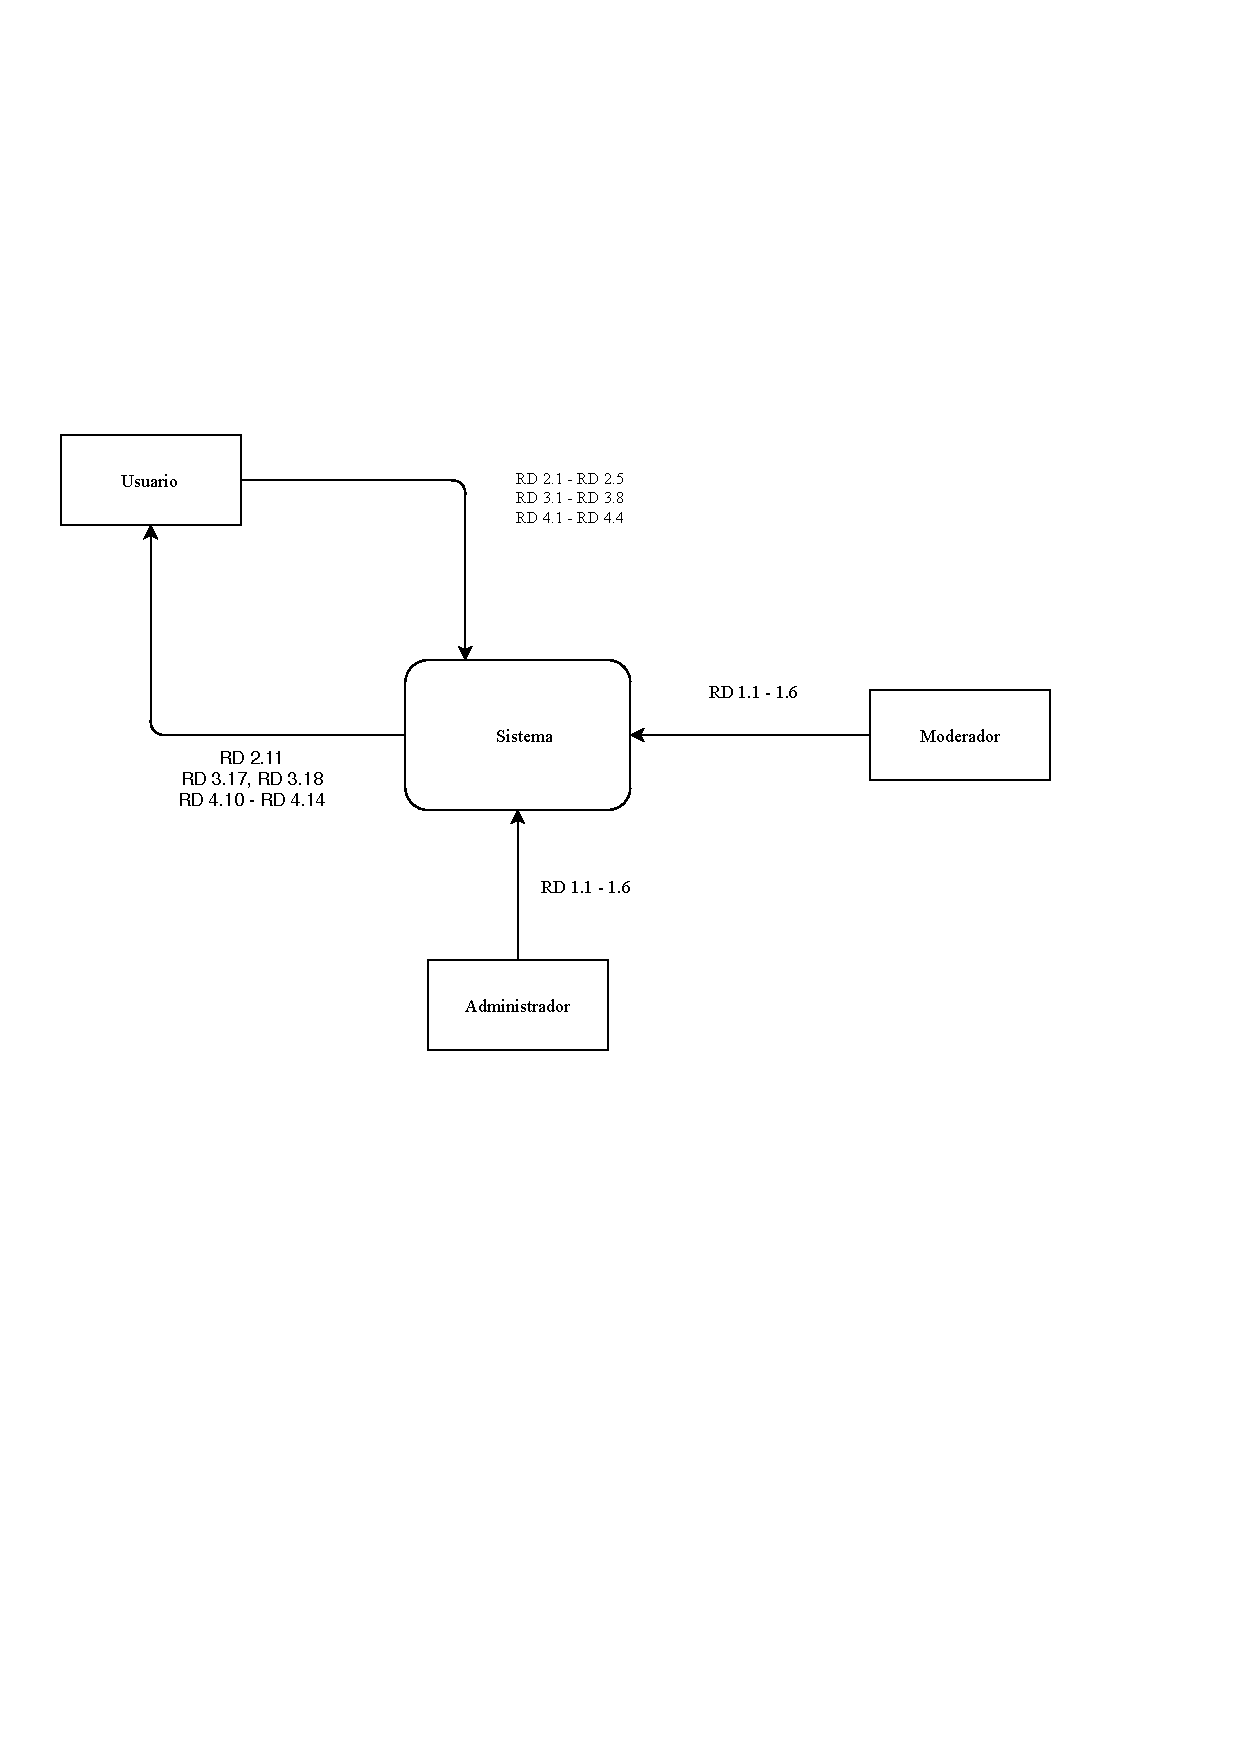
\includegraphics{diagramas/Caja_negra.pdf}
\end{figure}

\subsection{Esquema armazón}

\begin{figure}[H]
  \centering
  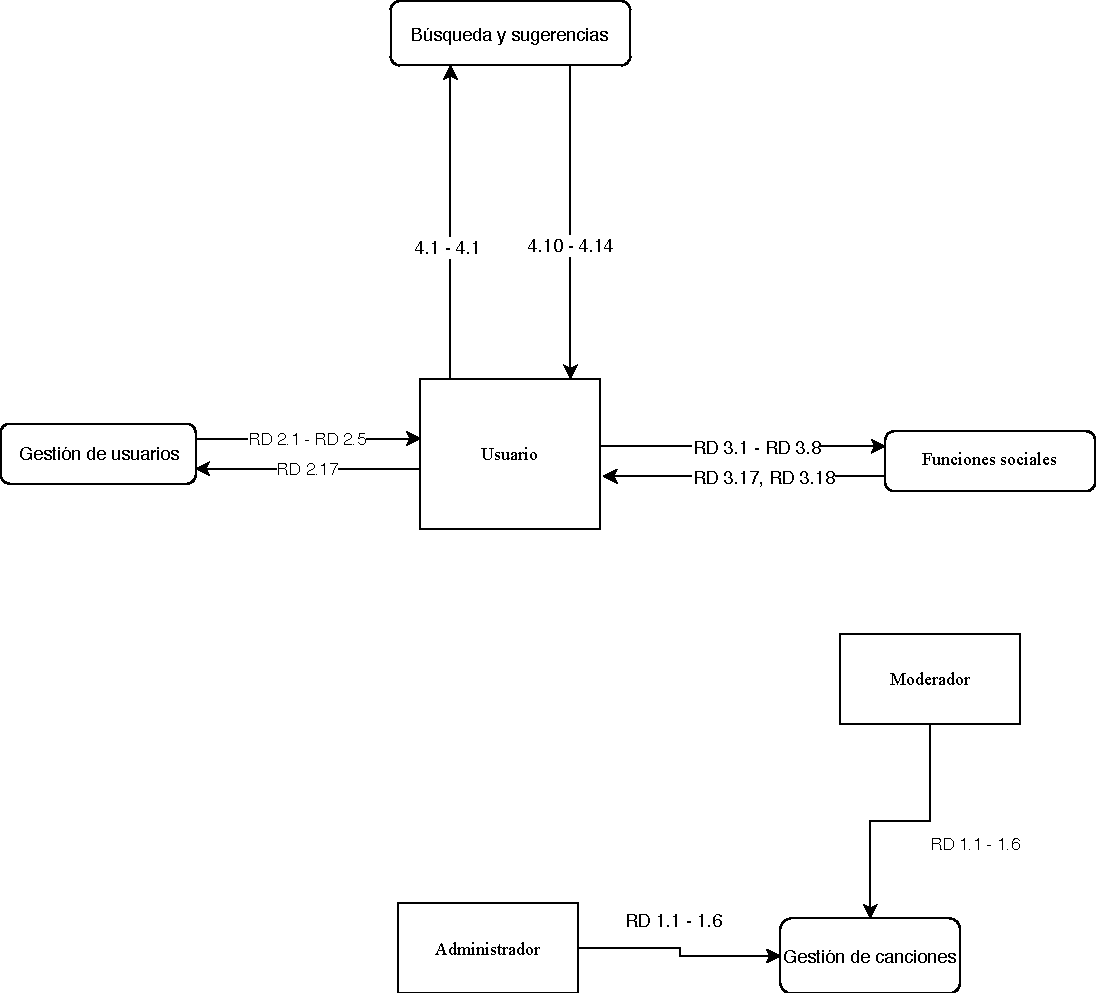
\includegraphics[scale=0.9]{diagramas/Esquema_armazon.pdf}
\end{figure}

\subsection{Refinamientos de los subsistemas}

\begin{figure}[H]
  \caption{Refinamiento del subsistema social}
  \centering
  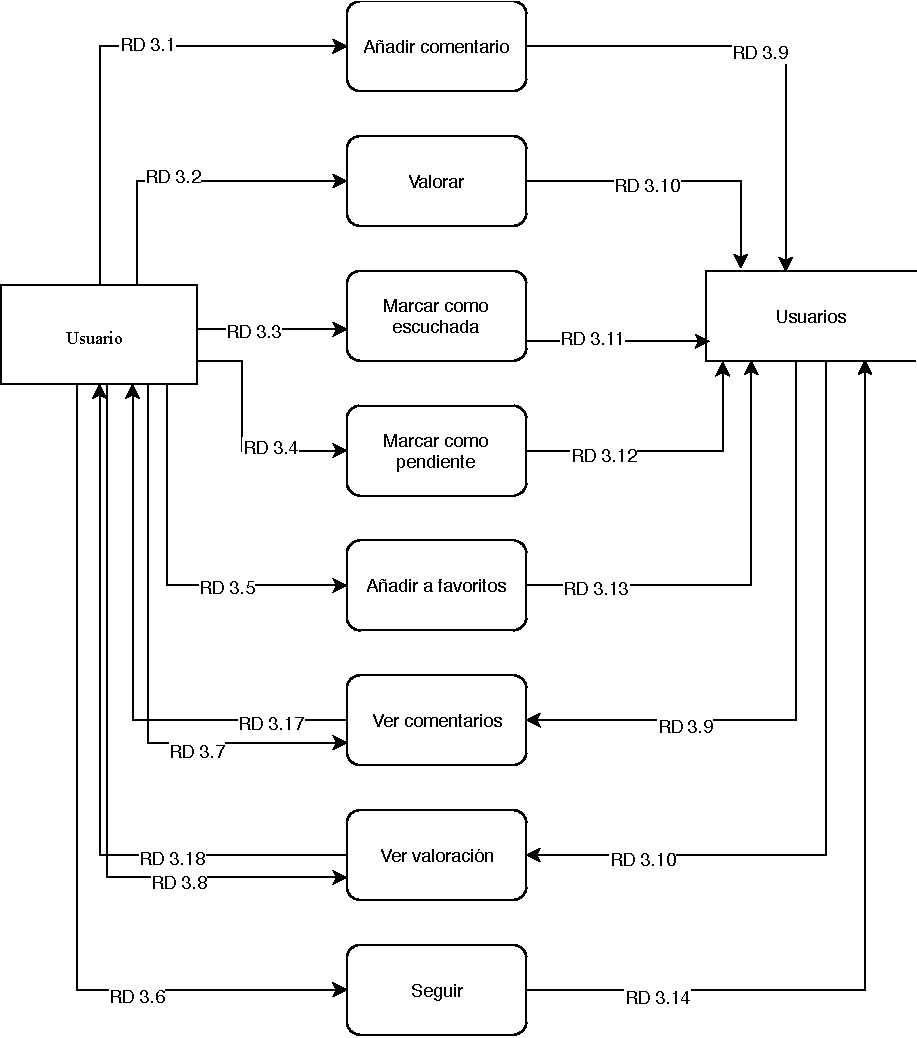
\includegraphics{diagramas/ref-social.pdf}
\end{figure}

\begin{figure}[H]
  \caption{Refinamiento del subsistema de búsquedas y sugerencias}
  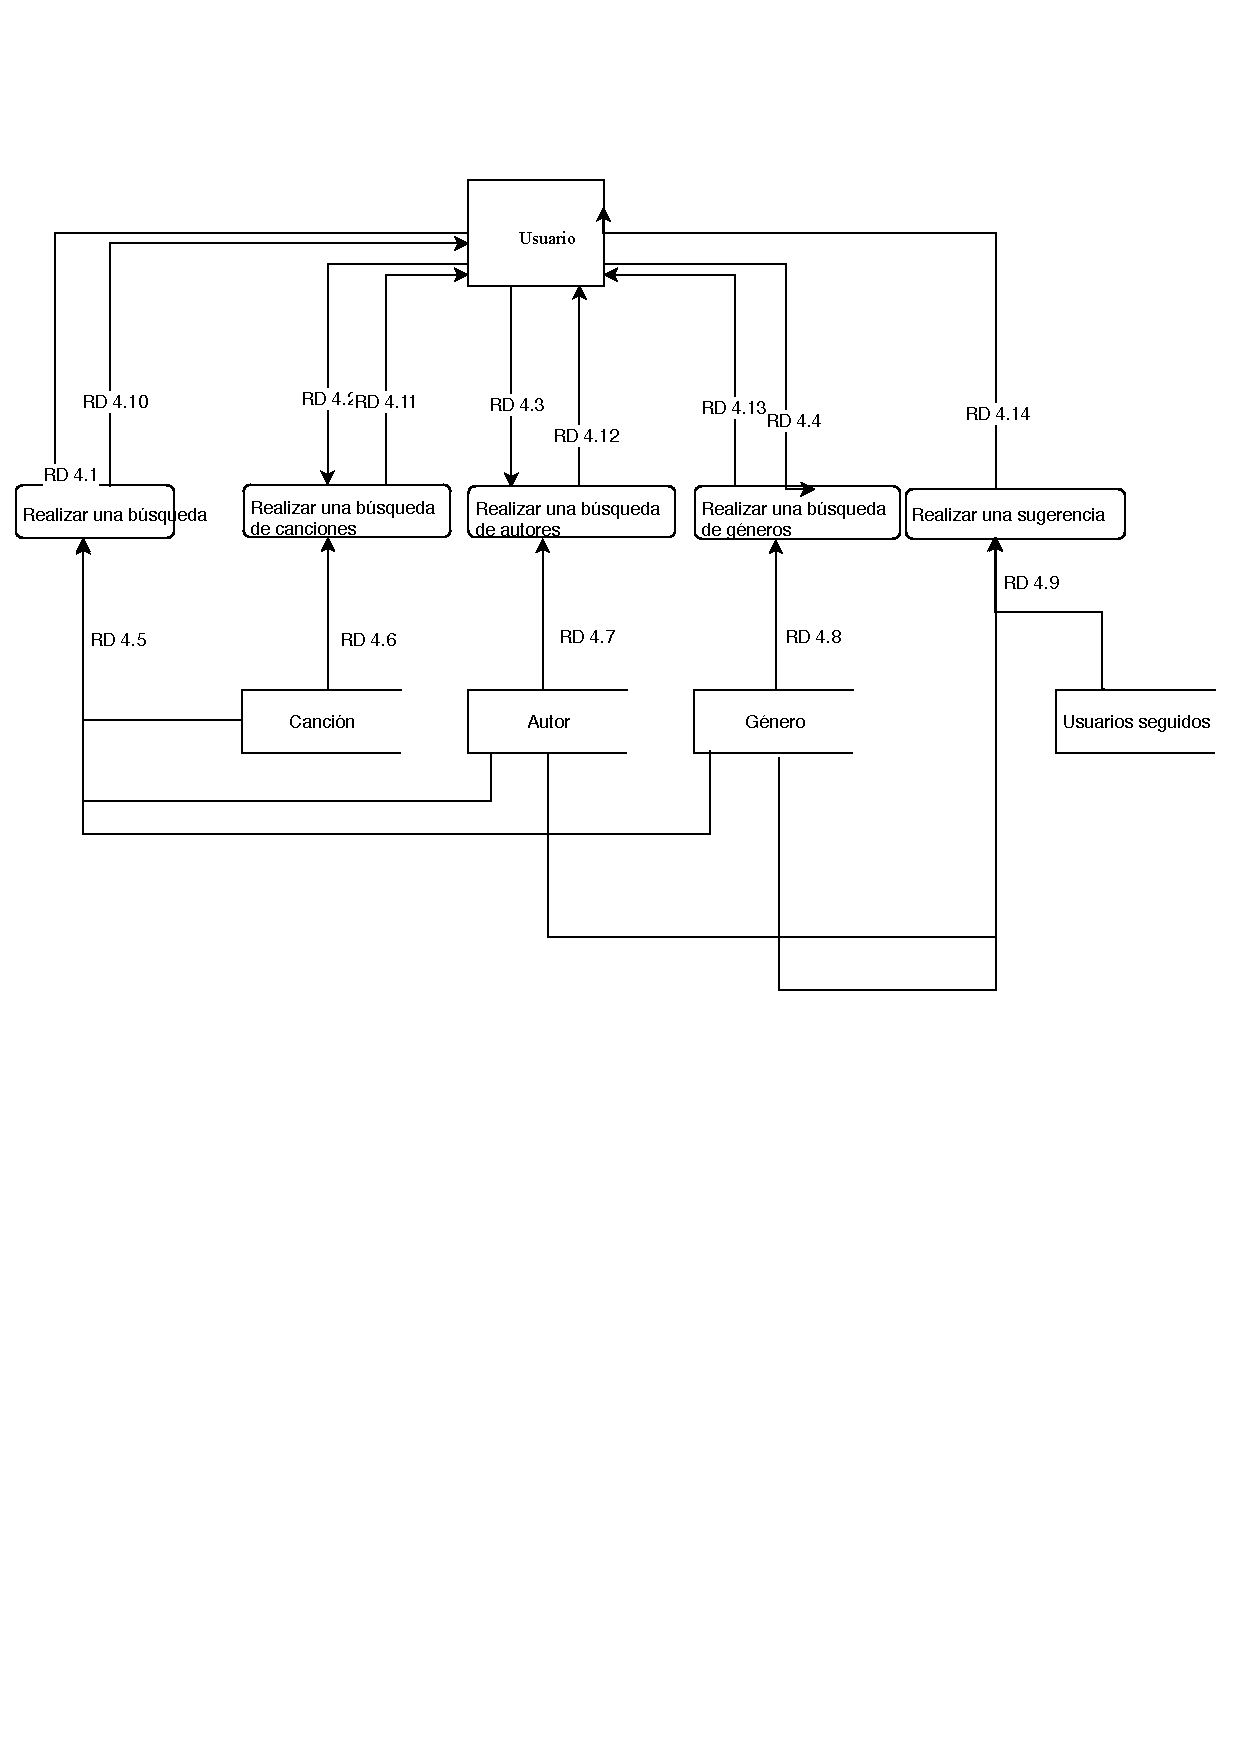
\includegraphics[scale=0.85]{diagramas/busqueda_refinamiento.pdf}
\end{figure}

\subsection{Esquemas externos}

\begin{figure}[H]
  \caption{Esquemas externos del subsistema social}
  \centering
  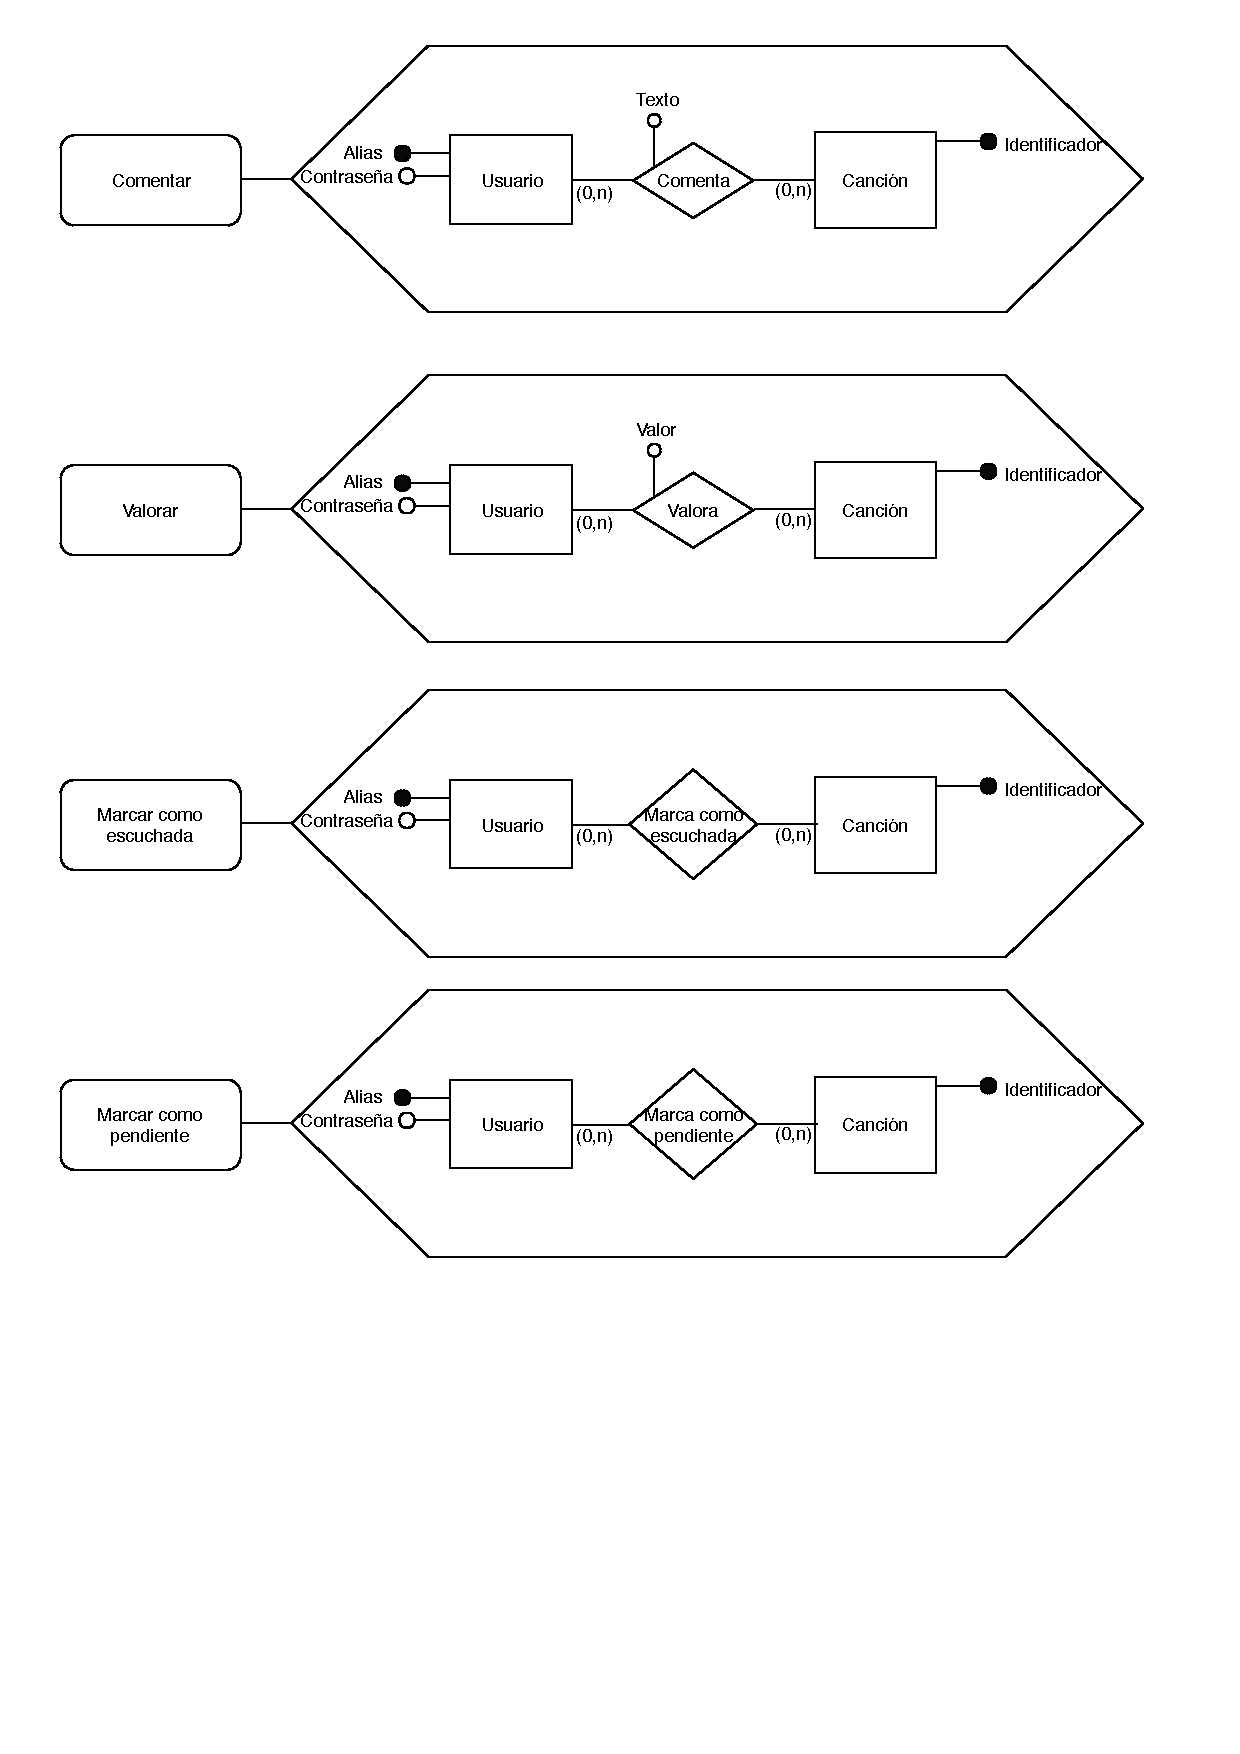
\includegraphics[scale=0.6]{diagramas/Esq-ext-social.pdf}
\end{figure}

\begin{figure}[H]
  \caption{Esquemas externos del subsistema de búsquedas y sugerenicas}
  \centering
  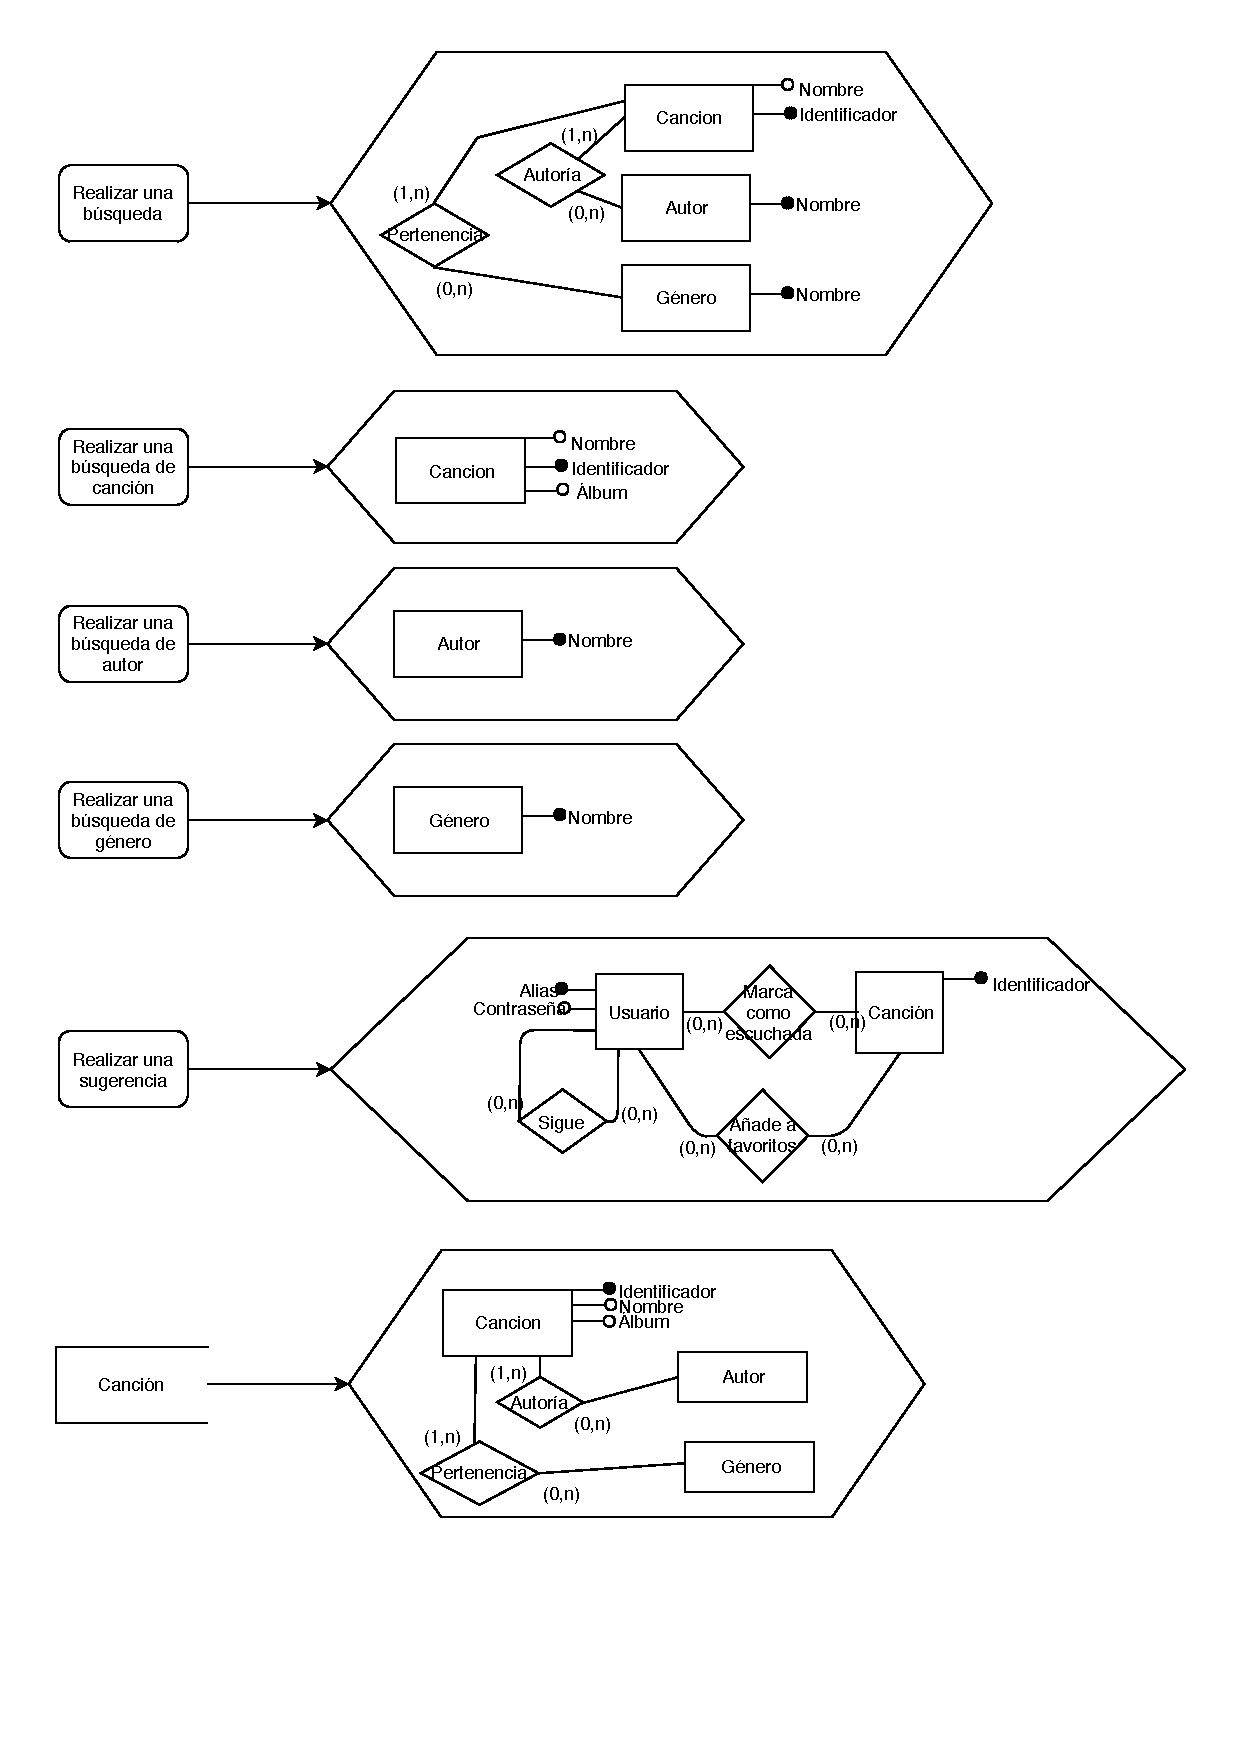
\includegraphics[scale=0.8]{diagramas/busqueda_esquema_externo.pdf}
\end{figure}

\subsection{Diagrama conceptual}

\begin{figure}[H]
  \caption{Diagrama conceptual del subsistema social}
  \centering
  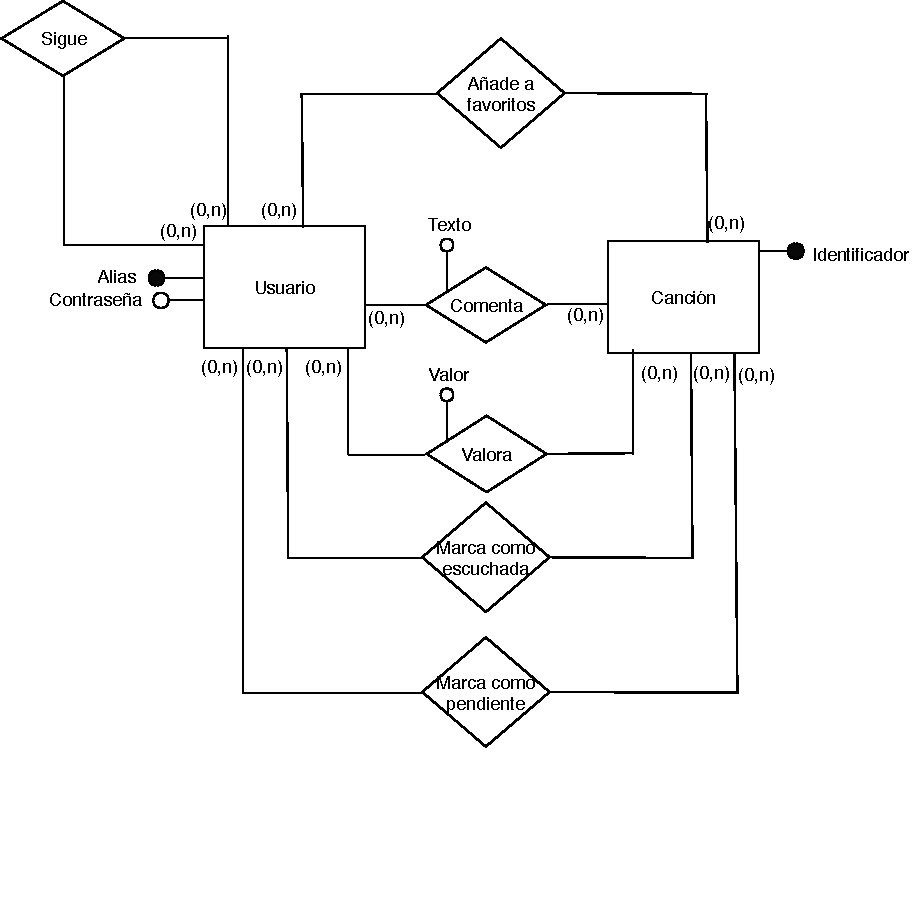
\includegraphics{diagramas/conceptual-social.pdf}
\end{figure}

\begin{figure}[H]
  \caption{Diagrama conceptual del subsistema de búsquedas y sugerencias}
  \centering
  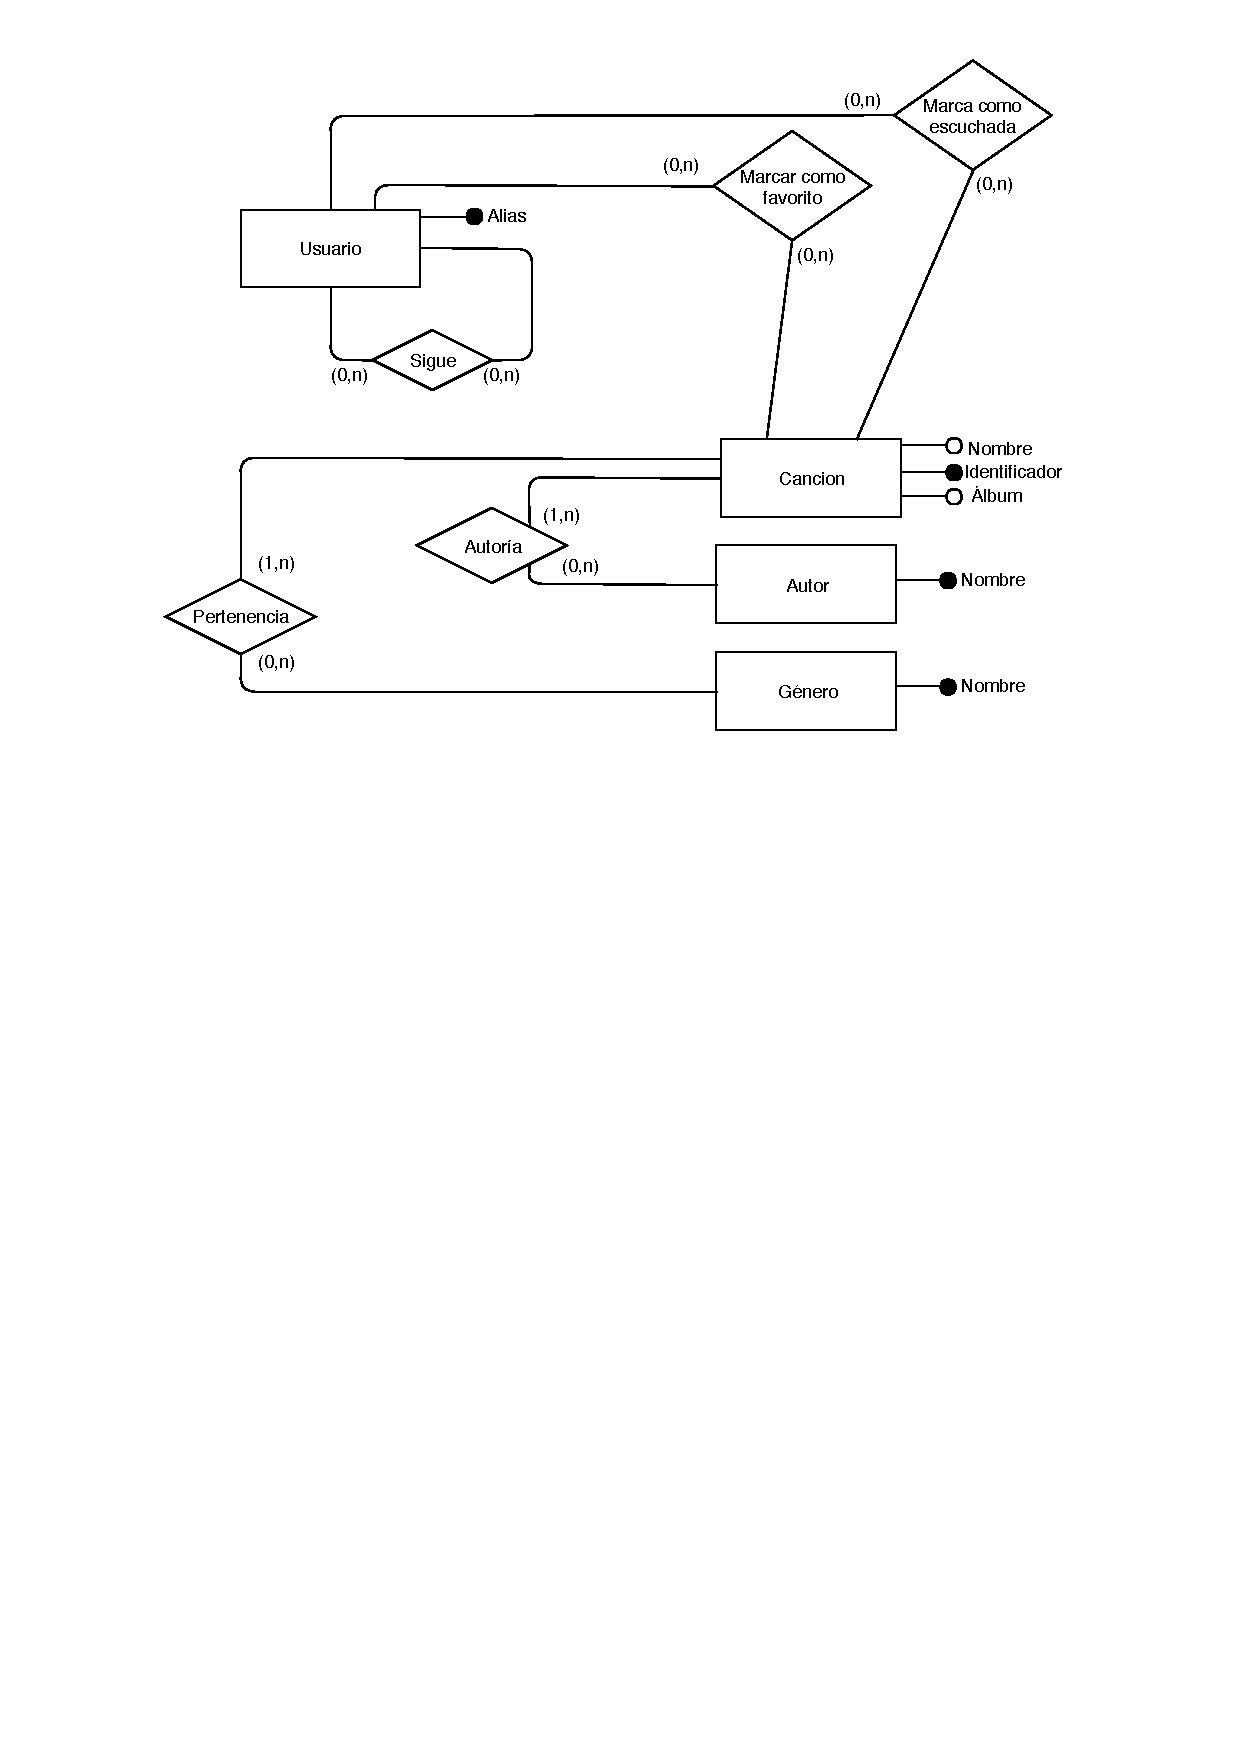
\includegraphics{diagramas/busqueda_modelo_conceptual.pdf}
\end{figure}

\subsection{Modelo entidad/relación}
